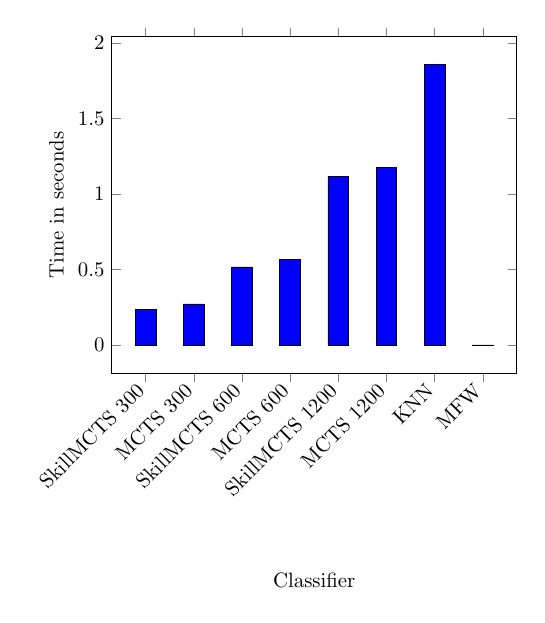
\begin{tikzpicture}[scale=0.75]
    \begin{axis}[
      symbolic x coords={SkillMCTS 300, MCTS 300, SkillMCTS 600, MCTS 600, SkillMCTS 1200, MCTS 1200, KNN, MFW},
      xtick=data,
      xlabel={Classifier},
      ylabel={Time in seconds},
      xlabel style={yshift=-1cm},
      ybar,
      x tick label style={font=\normalsize, rotate=45, anchor=east}]
      \addplot[ybar,fill=blue] coordinates {
           (SkillMCTS 300, 0.2379334)
           (MCTS 300, 0.2715728)
           (SkillMCTS 600, 0.5162254)
           (MCTS 600, 0.5665983)
           (SkillMCTS 1200, 1.1155539)
           (MCTS 1200, 1.1741404)
           (KNN, 1.8548495)
           (MFW, 0.000104)
        };
    \end{axis}
\end{tikzpicture}